
\chapter{Resultados} % Main chapter title
\label{Capitulo4}
\lhead{\emph{Resultados}}

\section{Imágenes obtenidas}
La Figura \ref{pics:originalHDR} muestra la imagen HDR captada por la cámara hiperespectral de donde fueron sacadas las diversas imágenes por longitud de onda espectral mostradas en la Figura \ref{pics:slices}. La toma fue adquirida mediante la utilización de la cámara hiperespectral que fue utilizada mediante el uso de un software especializado, controlando dicho aparato. La toma fue una sola, que captó un marco de visión a diversas longitudes de onda.
\begin{figure}[h]
\begin{center}
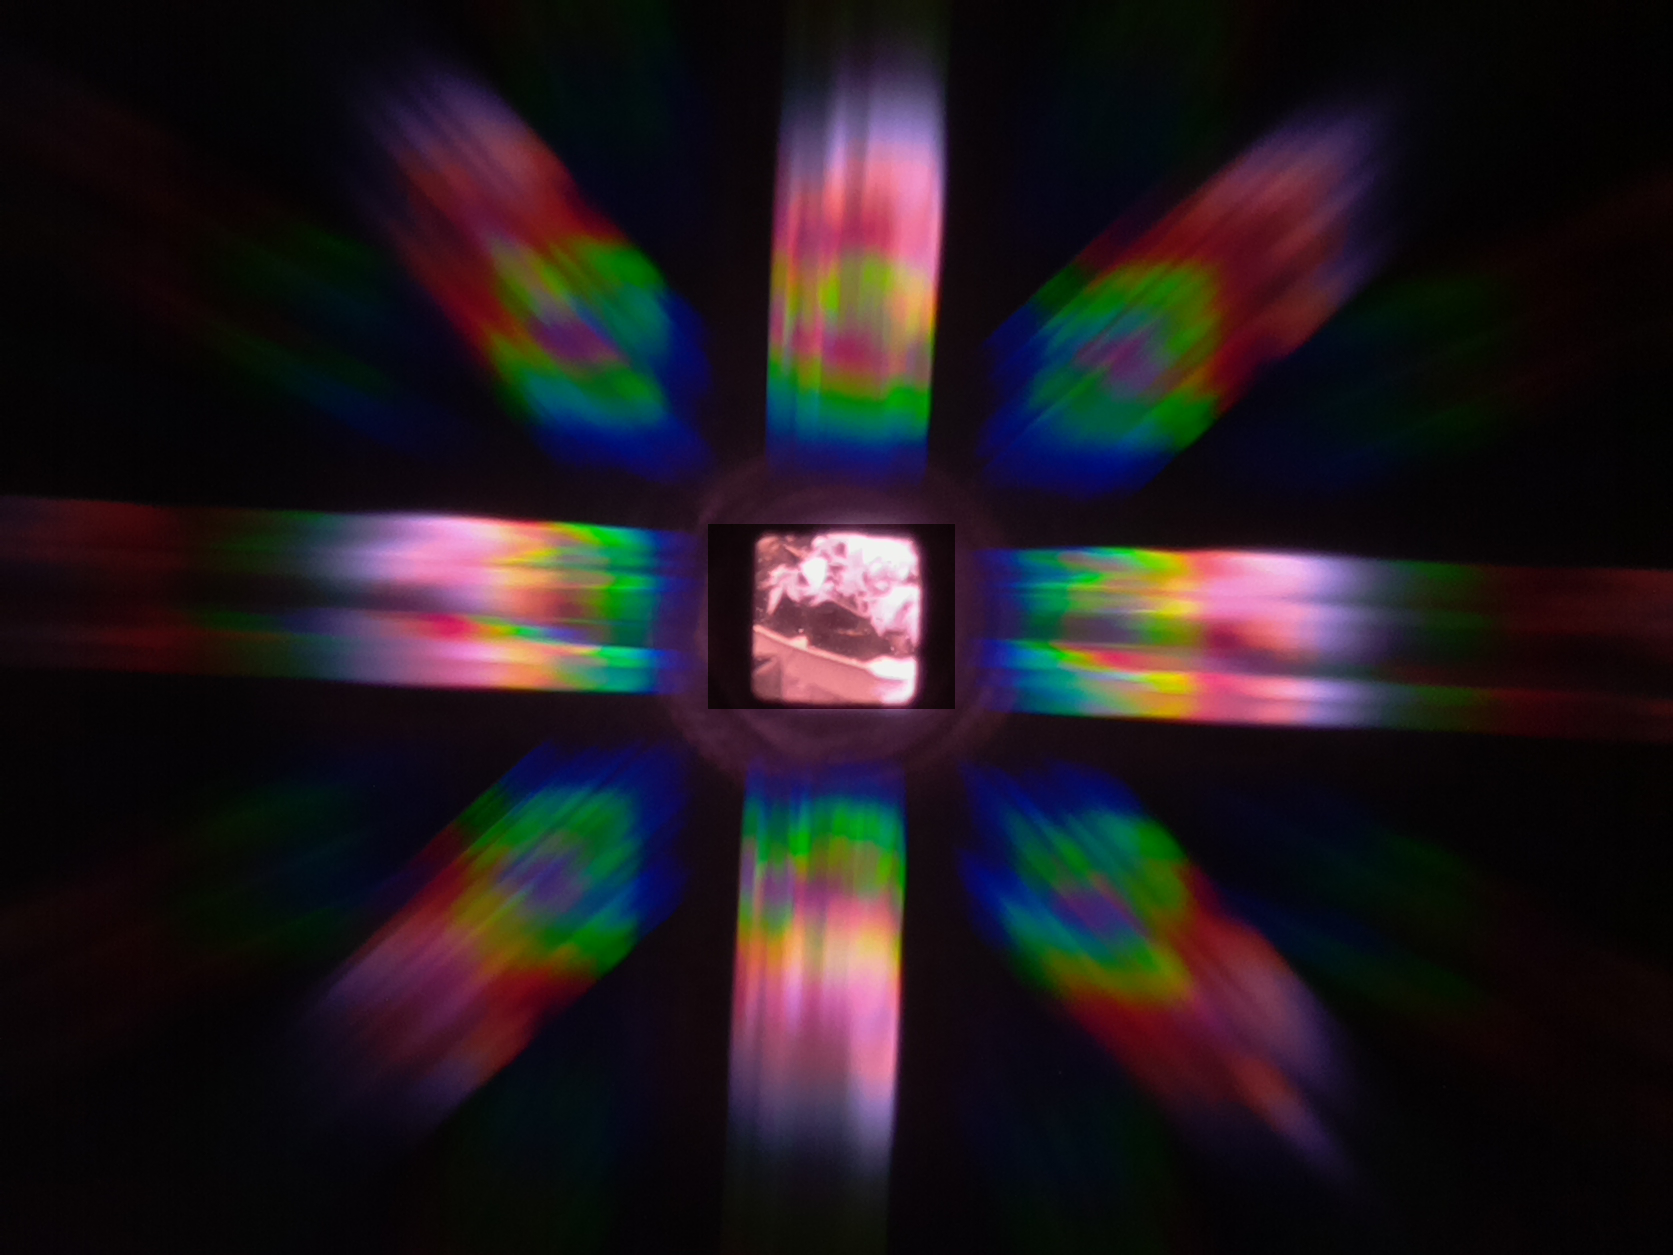
\includegraphics[scale=.3]{./images/RESULTS/original.png}
\end{center}
\caption{Imagen obtenida con camara hiperespectral.}
\label{pics:originalHDR}
\end{figure}

\begin{figure}[h]
\begin{center}$
\begin{array}{lll}
\subfloat[Imagen 466-637]{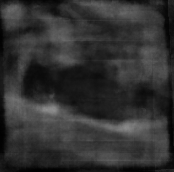
\includegraphics[scale=.99]{./images/RESULTS/slices/466.png}}&
\subfloat[Imagen 508-867]{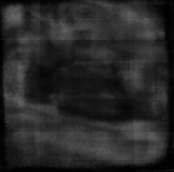
\includegraphics[scale=.99]{./images/RESULTS/slices/508.png}}&	
\subfloat[Imagen 549-087]{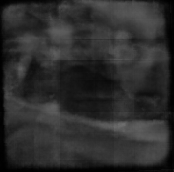
\includegraphics[scale=.99]{./images/RESULTS/slices/549.png}}
\end{array}$
\end{center}

\begin{center}$
\begin{array}{lll}
\subfloat[Imagen 589-307]{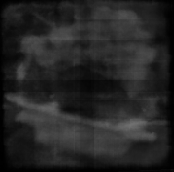
\includegraphics[scale=.99]{./images/RESULTS/slices/589.png}}&
\subfloat[Imagen 627-516]{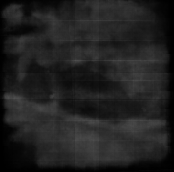
\includegraphics[scale=.99]{./images/RESULTS/slices/627.png}}&
\subfloat[Imagen 669-746]{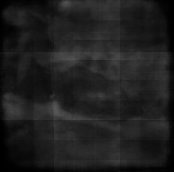
\includegraphics[scale=.99]{./images/RESULTS/slices/669.png}}
\end{array}$
\end{center}

\begin{center}$
\begin{array}{lll}
\subfloat[Imagen 709-966]{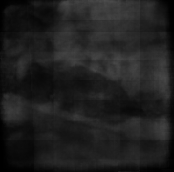
\includegraphics[scale=.99]{./images/RESULTS/slices/709.png}}&
\subfloat[Imagen 750-186]{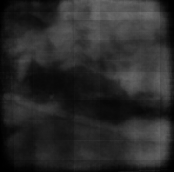
\includegraphics[scale=.99]{./images/RESULTS/slices/750.png}}&
\subfloat[Imagen 790-406]{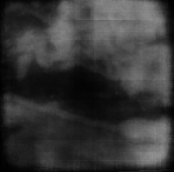
\includegraphics[scale=.99]{./images/RESULTS/slices/790.png}}
\end{array}$
\end{center}

\begin{center}$
\begin{array}{lll}
\subfloat[Imagen 830-625]{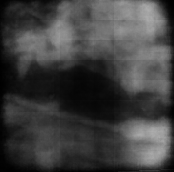
\includegraphics[scale=.99]{./images/RESULTS/slices/830.png}}&
\subfloat[Imagen 870-845]{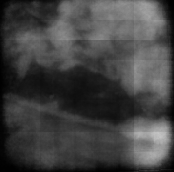
\includegraphics[scale=.99]{./images/RESULTS/slices/870.png}}&
\subfloat[Imagen 911-065]{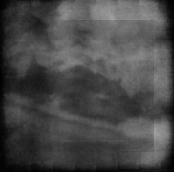
\includegraphics[scale=.99]{./images/RESULTS/slices/911.png}}
\end{array}$
\end{center}
\caption{Slices originales.}
\label{pics:slices}
\end{figure}

\clearpage
Con base en la Figura \ref{pics:squeme} los resultados tomados en consideración fueron el "Dau" que consta en aplicarle a los slices (conjunto de imágenes obtenidas mediante el método de obtención de imágenes por espectro CTIS) de la imagen hiperespectral el filtro utilizando la teoría de Daubichies (cápitulo \ref{rDau}), el MSB que consiste en la aplicación a la imagen original el Mosaic-Malvar y a ese resultado convertir la imagen HDR en slices para posterior aplicarle el Blur-Sharpened, además el MBS que de igual manera comienza aplicando el método de Moisac-Malvar seguido por el Blur-Sharpened y a ello después sacar los slices de la imagen hiperespectral, también el BSM que constaba en aplicarle a la imagen original el Blur-Sharpened seguido de sacar los slices y a ellos aplicarle el Mosaic-Malvar y por final se tomó el resultado BMS que era aplicarle a la imagen original el Bayer-Shapened y a ese resultado el Mosaic-Malvar para sacar los slices de la imagen superposicionada.

Para comparar los resultados se tomaron solo la imagen 870-845. Dichos resultados se muestran en la Figura \ref{pics:comparation}.

\begin{figure}[h]
\begin{center}$
\begin{array}{lll}
\subfloat[Original]{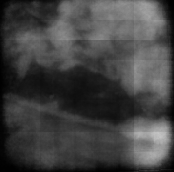
\includegraphics[scale=.99]{./images/RESULTS/compare870/original.png}}&
\subfloat[Dau]{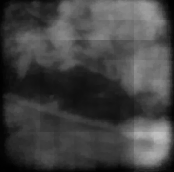
\includegraphics[scale=.7419]{./images/RESULTS/compare870/Dau.png}}&
\subfloat[MSB]{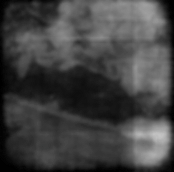
\includegraphics[scale=.7419]{./images/RESULTS/compare870/MSB.png}}
\end{array}$
\end{center}

\begin{center}$
\begin{array}{lll}
\subfloat[MBS]{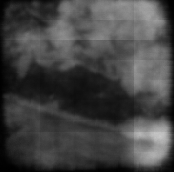
\includegraphics[scale=.99]{./images/RESULTS/compare870/MBS.png}}&
\subfloat[BSM]{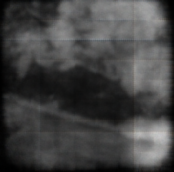
\includegraphics[scale=.7419]{./images/RESULTS/compare870/BSM.png}}&
\subfloat[BMS]{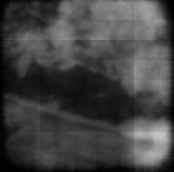
\includegraphics[scale=.99]{./images/RESULTS/compare870/BMS.png}}
\end{array}$
\end{center}

\caption{Comparación de resultados en imagen 870-845.}
\label{pics:comparation}
\end{figure}

Los resultados por los que se fueron obteniendo las imagenes se muestran en la Figura \ref{pics:process}, donde la imagen M es la imagen HDR original sometida a Malvar, MS es el resultado anterior sometido a el procedimiento de extracción de cubos. De ahí los slices se somente a Blur y sharpened resultando la imagen a comparar MSB. Y para finalizar el procedimiento se somete a la transformadas Daubichies para un último filtro dando como resultado la imagen MSBD.

\begin{figure}[h]
\begin{center}
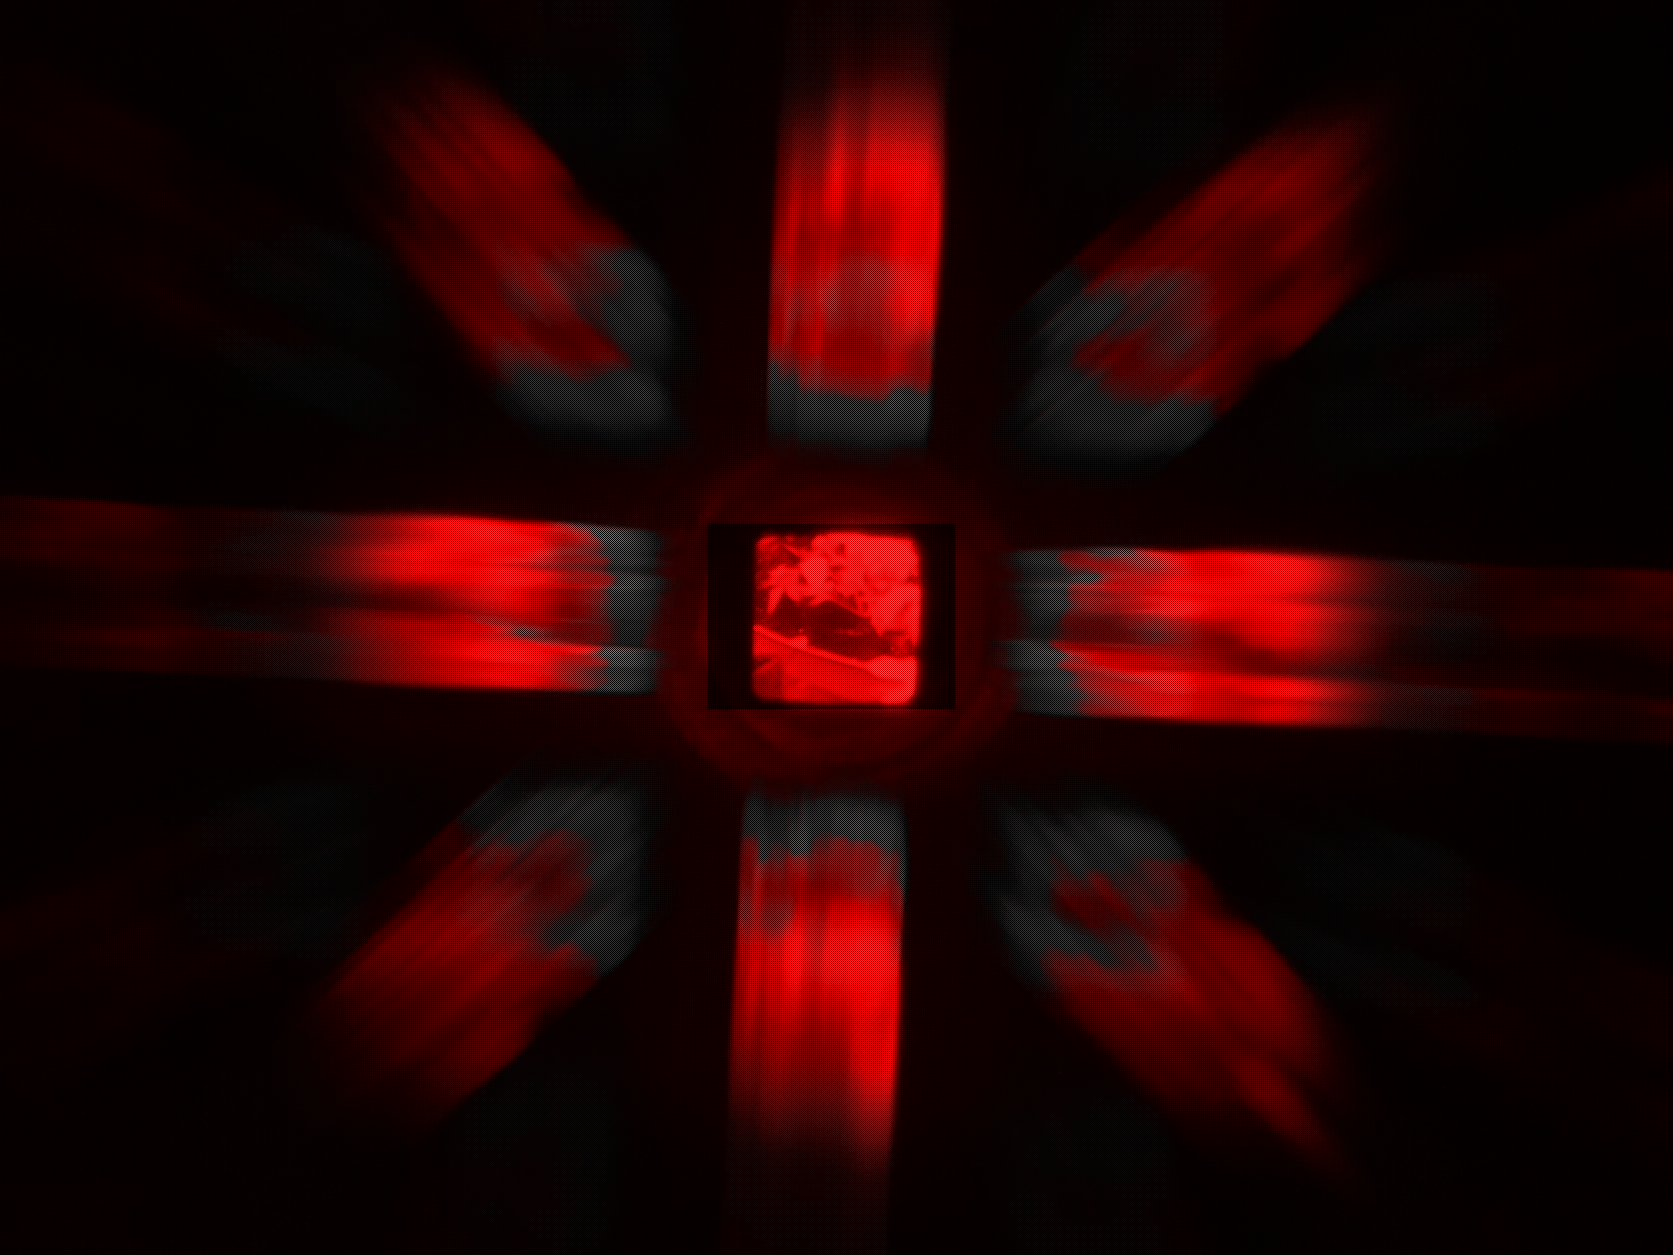
\includegraphics[scale=.2256]{./images/RESULTS/Malvar/mosaic.png}
\end{center}
\caption{Imagen obtenida con camara hiperespectral.}
\label{pics:originalHDR}
\end{figure}

\clearpage
\begin{figure}[h]
\begin{center}$
\begin{array}{lll}
\subfloat[MS]{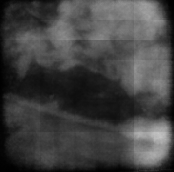
\includegraphics[scale=1.5]{./images/RESULTS/compare870/MS.png}}
\end{array}$
\end{center}

\begin{center}$
\begin{array}{lll}
\subfloat[MSB ]{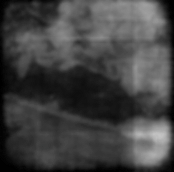
\includegraphics[scale=1.1]{./images/RESULTS/compare870/MSB.png}}&
\subfloat[MSBD]{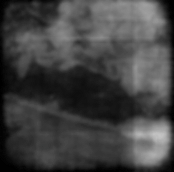
\includegraphics[scale=1.1]{./images/RESULTS/compare870/MSBD.png}}
\end{array}$
\end{center}

\caption{Proceso para MSBD en extracción 870-845.}
\label{pics:process}
\end{figure}
En las imágenes se muestran los resultados con base en los procedimientos explicados en el capítulo \ref{Capitulo2} y presentados en la Figura \ref{pics:squeme}.